% A note beside the APP1 report, on solving the maze with the region tree the
% generator already builds instead of with a graph search. It stands alone:
% the report does not depend on it, and it borrows only the shared preamble.
\documentclass[11pt,a4paper]{article}
% Everything the document needs before the first section: packages, page setup,
% the theorem and pseudocode environments, the drawing styles shared by every
% figure, and the notation macros. Sections and figures declare nothing of their
% own, so one edit here restyles the whole report.

\usepackage[T1]{fontenc}
\usepackage[utf8]{inputenc}
\usepackage{lmodern}
\usepackage[english]{babel}
\usepackage{microtype}
\usepackage{geometry}
\geometry{margin=2.4cm}

\usepackage{amsmath,amssymb,amsthm}
\usepackage{booktabs}
\usepackage{enumitem}
\usepackage{caption}
\usepackage{subcaption}
\usepackage{xcolor}
\usepackage[linesnumbered,ruled,vlined]{algorithm2e}
\usepackage{tikz}
\usetikzlibrary{arrows.meta,calc,fit,positioning,backgrounds}
\usepackage{import}
\usepackage{hyperref}
\usepackage{bookmark}

% --- Shared palette ------------------------------------------------------
% Named by the role each colour plays in a figure, not by the colour itself,
% so a change of palette does not turn every caption into a lie.
\definecolor{linkblue}{HTML}{1F4E79}
\definecolor{doorgreen}{HTML}{2E7D32}   % an edge kept: a door
\definecolor{wallred}{HTML}{C62828}     % an edge deleted: a wall segment
\definecolor{cellgrey}{HTML}{ECEFF1}    % the area a region covers
\definecolor{exitorange}{HTML}{E65100}  % the single exit cell

\hypersetup{colorlinks=true,linkcolor=linkblue,citecolor=linkblue,urlcolor=linkblue}

% --- Shared drawing styles ----------------------------------------------
\tikzset{
  cell/.style     = {draw=black!45, fill=cellgrey, minimum size=9mm},
  node vertex/.style = {circle, draw=black!70, fill=white, inner sep=0pt,
                        minimum size=4.2mm, font=\scriptsize},
  exit vertex/.style = {node vertex, draw=exitorange, very thick,
                        fill=exitorange!12},
  door/.style     = {doorgreen, line width=1.1pt},
  wall/.style     = {wallred, line width=1.1pt, dash pattern=on 2pt off 2pt},
  wall segment/.style = {wallred, line width=1.6pt},
  region/.style   = {draw=black!60, fill=cellgrey, thick},
  link/.style     = {-{Stealth[length=2mm]}, black!65},
  tree node/.style = {draw=black!70, rounded corners=1.5pt, inner sep=2.5pt,
                      font=\scriptsize, fill=white},
  tree leaf/.style = {tree node, draw=doorgreen!80!black, fill=doorgreen!8},
  tree edge/.style = {black!55},
}

% --- Theorem-like environments ------------------------------------------
\theoremstyle{definition}
\newtheorem{definition}{Definition}
\theoremstyle{plain}
\newtheorem{proposition}{Proposition}
\theoremstyle{remark}
\newtheorem*{remark}{Remark}

% --- Notation ------------------------------------------------------------
% The report says "the grid graph" and "the maze" constantly; these keep the
% symbols identical in prose, in displays and in pseudocode.
\newcommand{\gridgraph}{G_{\text{grid}}}
\newcommand{\gridedges}{E_{\text{grid}}}
\newcommand{\maze}{M}
\newcommand{\cells}{V}
\newcommand{\region}[2]{[#1]\times[#2]}
\newcommand{\exitcell}{v_{\text{exit}}}
\SetKwProg{Fn}{Function}{:}{}


% Only this note plots, so pgfplots is loaded here rather than in the shared
% preamble the report also reads.
\usepackage{pgfplots}
\pgfplotsset{compat=1.18}

\title{Solving the maze on its region tree\\
       \large a note beside the APP1 report}
\author{Mohamed Ali Tewfik Hamlil\\[2pt]
  \small M1 Artificial Intelligence, Universit\'e Grenoble Alpes}
\date{\today}

\begin{document}
\maketitle

\begin{abstract}
The report answers Problem~2 with Dijkstra's algorithm on the maze graph, which
settles $83$--$89\%$ of the cells at every size measured. That is more than the
problem requires. The generator already builds a binary tree of regions, and
that tree decides where the route goes without any cell being examined: a
division contributes a door to the route exactly when it separates the two
endpoints. Reading the route off the tree costs $\Theta(n^{0.68})$ node visits
against Dijkstra's $\Theta(n)$, and $O(\log n)$ extra memory against
$\Theta(n)$. This note states the lemma, gives the algorithm, derives the
exponent from a branching recurrence, and measures the one parameter that
recurrence needs.
\end{abstract}

\section{The question}

Every search in the report settles a large fraction of the maze. At
$256\times256$ cells Dijkstra settles $54\,293$ of $65\,536$, and A* with the
Manhattan estimate settles $52\,085$ --- a saving of $4\%$ on a problem whose
answer is a route of about $4\,300$ steps.

That is the wrong order of magnitude, and the reason is that the search is told
nothing about how the maze was built.

\begin{keypoint}
The generator does not merely produce a maze. It produces a \keyterm{binary tree
of regions}, and that tree records exactly where the walls are. A search that
reads it need not look at the maze at all.
\end{keypoint}

\section{The separation lemma}

Write $R$ for an internal node of the region tree, $R_\ell$ and $R_r$ for its
two children, and $(u,v)$ for its door, with $u\in R_\ell$ and $v\in R_r$.

\begin{proposition}[Separation]
\label{prop:separation}
Let $a,b$ be cells of $R$. The unique route from $a$ to $b$ crosses the door
$(u,v)$ \emph{if and only if} $a$ and $b$ lie in different children of $R$.
\end{proposition}

\begin{proof}
The correctness proof of the generator establishes that $(u,v)$ is the only edge
of the maze between $R_\ell$ and $R_r$, and that each child is spanned by a tree
of its own.

If $a$ and $b$ lie in different children, any route between them leaves one and
enters the other, so it uses an edge between them; $(u,v)$ is the only one.

If both lie in the same child, that child's own spanning tree already contains a
route between them. The maze is a tree, so its route between two cells is
unique, and therefore that one. It stays inside the child and does not touch
$(u,v)$.
\end{proof}

Figure~\ref{fig:separation} is the two cases. The test is a comparison of
coordinates against a rectangle --- no cell is visited, no neighbour list is
read.

% The separation lemma in one picture: the door of a division is on the route
% exactly when that division puts the two endpoints on opposite sides.
\begin{figure}[htbp]
  \centering
  \begin{subfigure}[b]{0.47\textwidth}\centering
    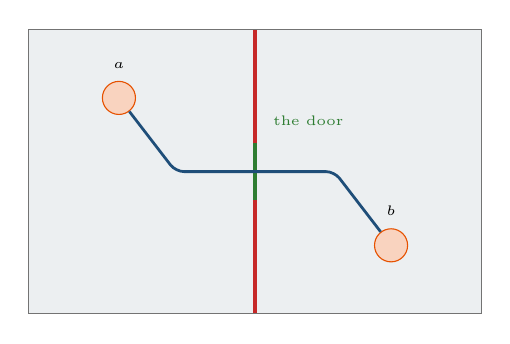
\begin{tikzpicture}[scale=0.72]
      \fill[cellgrey] (0,0) rectangle (8,5);
      \draw[black!55] (0,0) rectangle (8,5);
      \draw[wall segment] (4,0) -- (4,2);
      \draw[wall segment] (4,3) -- (4,5);
      \draw[door] (4,2) -- (4,3);
      \node[node vertex, fill=exitorange!25, draw=exitorange] (a) at (1.6,3.8) {};
      \node[node vertex, fill=exitorange!25, draw=exitorange] (b) at (6.4,1.2) {};
      \node[font=\tiny, above=1pt] at (a.north) {$a$};
      \node[font=\tiny, above=1pt] at (b.north) {$b$};
      \draw[linkblue, line width=1pt, rounded corners=3pt]
        (a) -- (2.6,2.5) -- (4,2.5) -- (5.4,2.5) -- (b);
      \node[font=\tiny, doorgreen, right] at (4.15,3.4) {the door};
    \end{tikzpicture}
    \caption{Opposite sides: the route \emph{must} cross, and the door is the
    only crossing there is. Recurse on both halves.}
    \label{fig:separated}
  \end{subfigure}\hfill
  \begin{subfigure}[b]{0.47\textwidth}\centering
    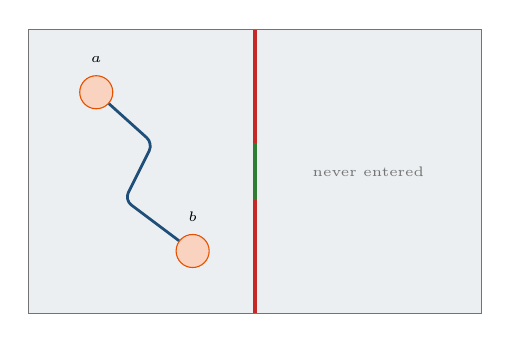
\begin{tikzpicture}[scale=0.72]
      \fill[cellgrey] (0,0) rectangle (8,5);
      \draw[black!55] (0,0) rectangle (8,5);
      \draw[wall segment] (4,0) -- (4,2);
      \draw[wall segment] (4,3) -- (4,5);
      \draw[door] (4,2) -- (4,3);
      \node[node vertex, fill=exitorange!25, draw=exitorange] (a) at (1.2,3.9) {};
      \node[node vertex, fill=exitorange!25, draw=exitorange] (b) at (2.9,1.1) {};
      \node[font=\tiny, above=1pt] at (a.north) {$a$};
      \node[font=\tiny, above=1pt] at (b.north) {$b$};
      \draw[linkblue, line width=1pt, rounded corners=3pt]
        (a) -- (2.2,3.0) -- (1.7,2.0) -- (b);
      \node[font=\tiny, black!55] at (6,2.5) {never entered};
    \end{tikzpicture}
    \caption{Same side: the route stays inside that half, and the other half is
    never looked at. Recurse once.}
    \label{fig:together}
  \end{subfigure}
  \caption{The separation lemma. Whether a division contributes a door to the
  route is decided by a containment test on its two children --- no cell of the
  maze is examined. The right-hand case is where the saving comes from: half the
  region is discarded in one step.}
  \label{fig:separation}
\end{figure}


\section{The algorithm}

\begin{algorithm}[H]
\caption{The route between two cells, read off the region tree.}
\label{alg:region-route}
\SetKwFunction{Route}{RouteInRegion}
\SetKwFunction{Holds}{Holds}
\KwIn{a region-tree node $R$, and two cells $a,b$ inside it.}
\KwOut{the number of doors between $a$ and $b$ (and, on the way, the route).}
\BlankLine
\Fn{\Route{$R$, $a$, $b$}}{
  \lIf{$R$ \textup{is a corridor leaf}}{\Return $|a_x-b_x|+|a_y-b_y|$}
  let $(u,v)$ be the door of $R$, with $u\in R_\ell$ and $v\in R_r$\;
  \lIf{$\Holds{$R_\ell$, $a$}$ \textup{\textbf{and}} $\Holds{$R_\ell$, $b$}$}{%
    \Return \Route{$R_\ell$, $a$, $b$}}
  \lIf{$\Holds{$R_r$, $a$}$ \textup{\textbf{and}} $\Holds{$R_r$, $b$}$}{%
    \Return \Route{$R_r$, $a$, $b$}}
  \tcp{separated: the door is on the route, by Proposition~\ref{prop:separation}}
  \lIf{$\Holds{$R_\ell$, $a$}$}{%
    \Return \Route{$R_\ell$, $a$, $u$} $+\,1+\,$ \Route{$R_r$, $v$, $b$}}
  \Return \Route{$R_r$, $a$, $v$} $+\,1+\,$ \Route{$R_\ell$, $u$, $b$}\;
}
\end{algorithm}

Correctness is Proposition~\ref{prop:separation} applied at every node, with the
corridor leaves as the base case: a corridor is a straight line, so the distance
inside it is the difference of coordinates.

Two properties are worth naming.

\begin{description}[leftmargin=*,style=nextline,itemsep=5pt]
  \item[A corridor costs one visit, not its length.] A leaf returns a run of
    cells as a single number. This is why the count below falls \emph{below} the
    length of the route it computes.
  \item[The maze is never read.] Only the region tree is. The neighbour lists of
    Section~2 of the report are not consulted at all.
\end{description}

\section{Why it is sublinear}

At each division, one of two things happens.

\begin{itemize}[leftmargin=*,itemsep=3pt]
  \item The endpoints are on the \keyterm{same side}. One recursive call, and
        half the region is discarded unexamined.
  \item They are \keyterm{separated}. Two recursive calls, one per half.
\end{itemize}

Write $p$ for the probability of the second. On a region of $m$ cells, each call
doing $O(1)$ work of its own,
\[
  T(m) \;=\; (1-p)\,T(m/2) \;+\; p\cdot 2\,T(m/2) \;+\; O(1)
        \;=\; (1+p)\,T(m/2)+O(1),
\]
and the master theorem gives

\begin{keypoint}
\[
  T(n)\;=\;\Theta\!\left(n^{\log_2(1+p)}\right).
\]
\end{keypoint}

The two endpoints of the scale are worth reading off. At $p=1$ --- every
division separating them --- the recurrence is $2T(n/2)$ and the cost is
$\Theta(n)$, no better than Dijkstra. At $p=0$ it is $T(n/2)$ and the cost is
$\Theta(\log n)$, a single root-to-leaf descent.

\begin{keypoint}
$\Theta(\log n)$ is therefore not available. It would require the endpoints
never to be separated, which happens only when they share a corridor.
$\log n$ is the cost of \keyterm{one} descent, and the search pays one descent
per separation.
\end{keypoint}

\section{Measuring \texorpdfstring{$p$}{p}}

The recurrence has one parameter, so it makes one prediction, and the prediction
is checkable. Sixty mazes per size, counting at every visited division whether
it recursed once or twice.

\begin{center}
\begin{tabular}{@{}lrrrrrr@{}}
  \toprule
  Endpoints & $n$ & Visits & One-way & Two-way & $p$ & $\log_2(1+p)$ \\
  \midrule
  far corners    & $1024$  & $115$  & $26.7$  & $43.9$  & $0.62$ & $0.70$ \\
  far corners    & $16384$ & $703$  & $171.8$ & $264.9$ & $0.61$ & $0.68$ \\
  far corners    & $65536$ & $1588$ & $388.1$ & $599.7$ & $0.61$ & $0.68$ \\
  \midrule
  uniform random & $1024$  & $73$   & --- & --- & $0.54$ & $0.63$ \\
  uniform random & $16384$ & $408$  & --- & --- & $0.58$ & $0.66$ \\
  uniform random & $65536$ & $950$  & --- & --- & $0.59$ & $0.67$ \\
  \bottomrule
\end{tabular}
\end{center}

The exponent fitted to the measured visits is $0.66$--$0.72$ for far corners,
against the $0.68$ the recurrence predicts from $p=0.61$. The two agree at every
size.

$p$ is not a constant of nature: it depends on where the endpoints are. Corners
are the hard case, since a division far from both is likelier to fall between
them; uniformly random endpoints give $p\approx0.58$ and a slightly smaller
exponent. Both are comfortably below $1$, which is what matters.

% Measured visits against area, on log-log axes, so that a power law is a
% straight line and its exponent is the slope.
\begin{figure}[htbp]
  \centering
  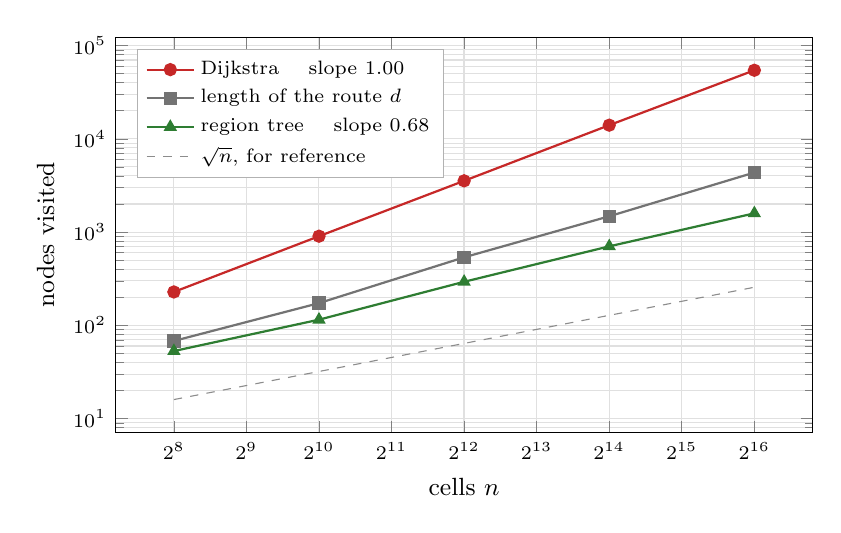
\begin{tikzpicture}
    \begin{loglogaxis}[
      width=0.86\textwidth, height=6.6cm,
      xlabel={cells $n$}, ylabel={nodes visited},
      log basis x=2, log basis y=10,
      legend pos=north west, legend cell align=left,
      legend style={font=\scriptsize, draw=black!30},
      grid=both, grid style={black!12},
      tick label style={font=\scriptsize}, label style={font=\small},
    ]
      \addplot[mark=*, wallred, thick] coordinates
        {(256,228) (1024,903) (4096,3543) (16384,13996) (65536,54293)};
      \addlegendentry{Dijkstra \quad slope $1.00$}
      \addplot[mark=square*, black!55, thick] coordinates
        {(256,68) (1024,173) (4096,536) (16384,1477) (65536,4348)};
      \addlegendentry{length of the route $d$}
      \addplot[mark=triangle*, doorgreen, thick] coordinates
        {(256,53) (1024,115) (4096,293) (16384,703) (65536,1588)};
      \addlegendentry{region tree \quad slope $0.68$}
      \addplot[dashed, black!45, no marks, domain=256:65536, samples=2]
        {sqrt(x)};
      \addlegendentry{$\sqrt{n}$, for reference}
    \end{loglogaxis}
  \end{tikzpicture}
  \caption{Both axes logarithmic, so a power law is a straight line and the
  exponent is its slope. Dijkstra runs parallel to $n$; the region-tree search
  runs at slope $0.68$, below even the length of the route it returns, because
  one visit to a corridor leaf covers a whole straight run.}
  \label{fig:growth}
\end{figure}


\section{What it costs, beside the alternatives}

\begin{center}
\begin{tabular}{@{}lrll@{}}
  \toprule
  Method & Visits at $n=65536$ & Time & Extra memory \\
  \midrule
  Dijkstra                    & $54\,293$ & $\Theta(n\log n)$   & $\Theta(n)$ \\
  A*, Manhattan               & $52\,085$ & $\Theta(n\log n)$   & $\Theta(n)$ \\
  \textbf{Region tree}        & $\mathbf{1\,588}$ & $\Theta(n^{0.68})$ & $O(\log n)$ \\
  \midrule
  Binary-tree maze, greedy walk & $510$   & $\Theta(\sqrt n)$   & $O(1)$ \\
  \bottomrule
\end{tabular}
\end{center}

The memory column is the sharper difference. Dijkstra needs a distance, a parent
and a settled flag for every cell before it starts. The region-tree search needs
only its own recursion stack, which is the depth of the tree.

The last row is a different maze, not a different search: the binary-tree
generator makes the Manhattan distance \emph{exact}, so the route is found by
walking north-or-west with no search at all. It is listed to show where the
scale ends --- and what it costs, since a maze solvable by always turning the
same way is barely a maze.

\section{What this would change in the report}

Section~2.8 of the report lists the region tree as feeding the cost analysis
only. On the evidence here it should feed the search as well, and the handout's
own learning objectives point that way: they ask for traversals of a binary tree
and for \emph{searching a path linking two nodes in a binary tree}, which is
Algorithm~\ref{alg:region-route} and not Dijkstra.

Two things would have to be said carefully if it were folded in.

\begin{itemize}[leftmargin=*,itemsep=3pt]
  \item The exponent $0.68$ is measured, and derived from a $p$ that is itself
        measured. It is not a worst-case bound: the worst case is
        $\Theta(n)$, when every division separates the endpoints.
  \item Returning the \emph{distance} costs $\Theta(n^{0.68})$; writing out the
        route cell by cell costs $\Theta(d)$ on top, because that is the size of
        the output. The compression is in the corridors, and it survives only as
        long as the answer stays compressed.
\end{itemize}

\end{document}
